\documentclass[11pt]{article}
    \usepackage{caption}
    \usepackage{graphicx}
    \usepackage{mathtools}
    \graphicspath{ {img/} }
    \setlength{\parindent}{0pt}
    \DeclareCaptionType{equ}[][]
    \usepackage[svgnames]{xcolor}
    \newcommand\tab[1][1cm]{\hspace*{#1}}    
    \newcommand*{\plogo}{\fbox{$\mathcal{BM}$}}
        
    \usepackage{PTSerif}
    
    \begin{document} 
        
    \begin{titlepage}
    
        \raggedleft
        
        \vspace*{\baselineskip}
        
        {\Large Bryan Melanson}
        
        \vspace*{0.167\textheight}
        
        \textbf{\LARGE How to Not Fail}\\[\baselineskip]
        
        {\textcolor{Red}{\Huge Control Systems}}\\[\baselineskip]
        
        {\Large \textit{While never going to class}}
        
        \vfill
        
        {\large Computer Engineering 2020 ~~\plogo}
        
        \vspace*{3\baselineskip}
    
    \end{titlepage}

    \pagebreak

    \tableofcontents

    \pagebreak

    \section{Modeling in the Frequency Domain}

    \pagebreak
    
    \section{Modeling in the Time Domain}
    
    \pagebreak
    
    \section{Time Response}
    
    \pagebreak
    
    \section{Reduction of Multiple Systems}
    
    \pagebreak

    \section{Stability}
    \subsection{Routh-Hurwitz Criteria}
    \subsection{Routh-Hurwitz Special Cases}
    
    \pagebreak

    \section{Steady State Errors}

    \textit{Steady State Error} is defined as the difference between the input and output as t $\rightarrow \infty$. When testing for factors such as constant position, constant velocity and constant acceleration, inputs such as unit steps $u(t)$, ramps $r(t)$ and parabolas are used. This discussion is limited to stable systems.\\
   
    \begin{center}
        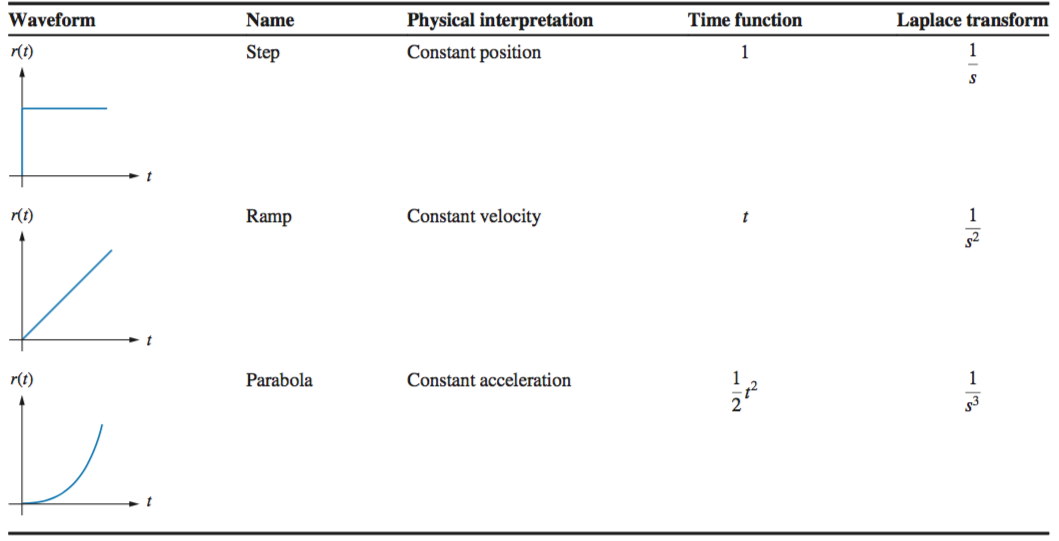
\includegraphics[width=300 px]{img/inputs} \\
    \end{center}

    Most steady state errors $E(s)$ arise from the input and/or the configuration of the system, as seen in the diagrams below for general closed loop and unity feedback systems.

    \begin{center}
        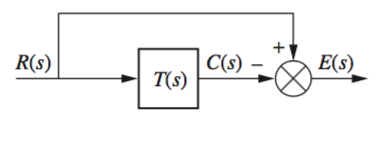
\includegraphics[width=300 px]{img/closedlooperror} \\
    \end{center}

    \begin{center}
        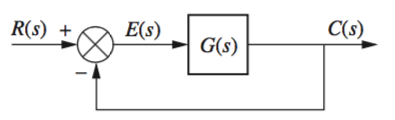
\includegraphics[width=300 px]{img/unityfeedback} \\
    \end{center}
    
    In the first case $E(s) = R(s) - C(s)$ is the error. If the input $R(s)$ is a step input, then $C(s)$ should $= R(s)$ and $E(s) = 0$. However, if gain $K$ is introduced, $C(s) = KR(s)$ and $E(s)$ must be finite and non-zero. \\
    
    \begin{center}
        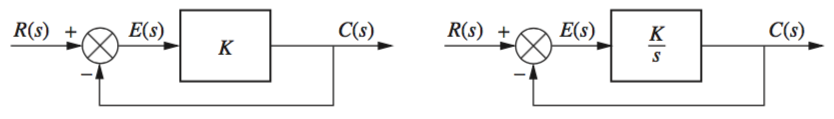
\includegraphics[width=300 px]{img/integrator} \\
    \end{center}

    From these systems we see that $C(s)$ = $KE(s)$, or $E(s) = \frac{1}{K}C(s)$

    \subsection{Steady State Error for Unity Feedback Systems}

    Steady-state error can be calculated from transfer function $T(s)$ or the open loop transfer function $G(s)$. Once $E(s)$ is found, the steady state error can be found using the \textit{Final Value Theorem}, which states that the value at infinity is equal to the Laplace as $s \rightarrow 0$.

    \begin{center}
        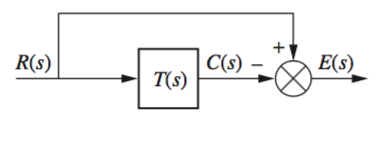
\includegraphics[width=300 px]{img/closedlooperror} \\
    \end{center}

    \begin{center}
        $E(s) = R(s) - C(s)$ \\
        $C(s) = R(s)T(s)$ \\ 
        $E(s) = R(s)[1 - T(s)]$ \\
        $e(\infty) = \text{lim}_{s\rightarrow \infty}  e(t) = \text{lim}_{s\rightarrow 0}  sE(s)$ \\ 
        $e(\infty) = \text{lim}_{s\rightarrow 0} sR(s)[1 - T(s)]$ \\
    \end{center}

    \subsubsection{Steady State Error in Terms of G(s)}

    The steady-state error for unit step inputs is \\ 

    $e(\infty) = \frac{1}{1 + \text{lim}_{s\rightarrow 0} G(s)}$ \\
    
    The steady-state error for ramp inputs of unit velocity is \\
    
    $e(\infty) = \frac{1}{\text{lim}_{s\rightarrow 0} sG(s)}$ \\

    The steady-state error for parabolic inputs of unit acceleration is \\
    
    $e(\infty) = \frac{1}{\text{lim}_{s\rightarrow 0} s^2G(s)}$ \\

    The terms in the denominator are known as $k_p, k_v, k_a$, the \textbf{static error constants}, representing position, velocity and acceleration, respectively. \\
    
    Systems can also be defined by \textbf{system type}. This defines the number of pure integrations in the forward path, assuming a unity feedback system. Increasing the system type decreases the steady-state error as long as the system is stable.

    \begin{center}
        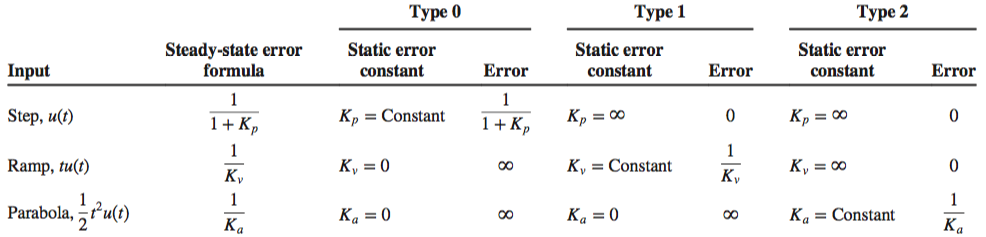
\includegraphics[width=300 px]{img/types} \\
    \end{center}

   The steady-state error is inversely proportional to the static error constant - the larger the constant, the smaller the steady-state erorr. Increasing gain increases the static error constant, thus, increasing the gain decreases the steady-state error if the system is stable.

    \pagebreak

    \section{Root Locus Techniques}

    The following sections apply to \textbf{Negative Feedback Closed Loop} systems.

    \subsection{Sketching the Root Locus}

    \subsubsection{Number of Branches}

    The number of branches in a root locus equal the number of poles.

    \subsubsection{Symmetry}

    The root locus is symmetrical about the real axis.

    \subsubsection{Real Axis Segments}

    On the real axis, for $K > 0$ the root locus exists to the left of an odd number of real-axis, finite open-loop poles and/or finite open-loop zeros.

    \subsubsection{Starting and Ending Points}

    The root locus begins at the finite and infinite poles of $G(s)H(s)$ and ends at the finite and infinite zeros of $G(s)H(s)$.

    \subsubsection{Behavior at Infinity}

    \begin{center}
    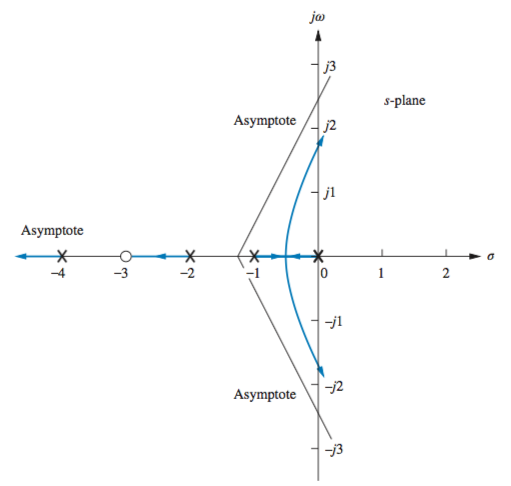
\includegraphics[width=300 px]{img/asymptotes} \\
    \end{center}

    \subsection{Refining the Sketch}

    \subsubsection{Breakaway/Break-in Point}

    At the breakaway or break-in point, the branches of the root locus form an angle of 180°/$n$ with the real axis, where $n$ is the number of closed-loop poles arriving at or departing from the single breakaway or break-in point on the real axis. These are the points when gain is at its minimum and maximum, respectively. \\
        
    For all points on the root locus, \\
    
    $K = -\frac{1}{G(s)H(s)}$, $\frac{1}{G(s)H(s)} = -1$ and by differential calculus, \\
    
    $K = -\frac{1}{G(\sigma)H(\sigma)}$ where breakpoints occur - setting $\sigma$ to 0 will produce $K$.

    \begin{center}
        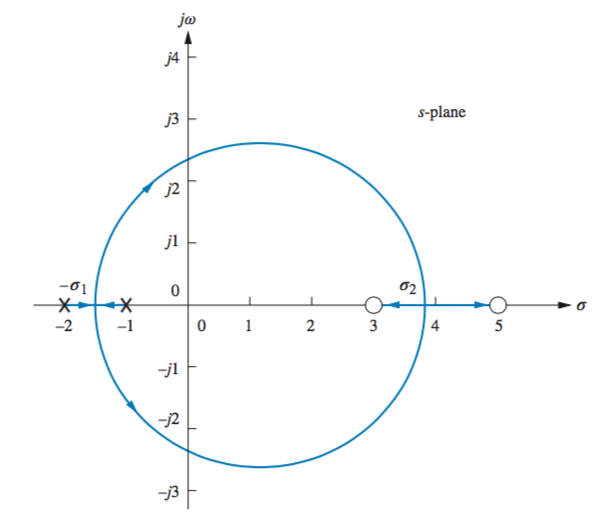
\includegraphics[width=300 px]{img/breakpoints} \\
    \end{center}

    Or, conversely, \\

    $\sum \frac{1}{\sigma + z_i} = \sum \frac{1}{\sigma + p_i}$ \\

    Where $z$ and $p$ are the zero and pole values. By equating the two sides and simplifying to a single equation, factoring can produce $\sigma$.

    \subsubsection{$j\omega$-Axis Crossings}

    The crossing of the $j\omega$ axis defines when the system becomes unstable. The crossing of the $\omega$ axis deines the frequency of oscillation, while the gain at the $j\omega$ axis yields the maximum positive gain for system stability. \\ 

    The $j\omega$ axis crossings can be found using the Routh-Hurwitz criterion. Forcing a row of zeros yields the gain, then going back a row and solving for the roots yields the frequency at the imaginary axis crossing.

    \subsubsection{Angles of Departure and Arrival}

    If we assume a point on the root locus $\epsilon$ close to a complex \textbf{pole}, the sum of angles drawn from all finite poles and zeros to this point is an odd multiple of 180$^\circ$. Except for the \textbf{pole} that is $\epsilon$ close to the point, we assume all angles drawn from all other poles and zeros are drawn directly to the \textbf{pole} that is near the point. Thus, the only unknown angle in the sum is the angle drawn from the \textbf{pole} that is $\epsilon$ close. We can solve for this unknown angle, which is also the angle of departure from this complex \textbf{pole}. \\

    $-\theta_1 + \theta_2 + \theta_3 - \theta_4 - \theta_5 + \theta_6 =…(2k+1)180^\circ$ \\ 
    
    \textit{or} \\ 

    $\theta_1 = \theta_2 + \theta_3 - \theta_4 - \theta_5 + \theta_6 -…(2k+1)180^\circ$ \\

    \begin{center}
        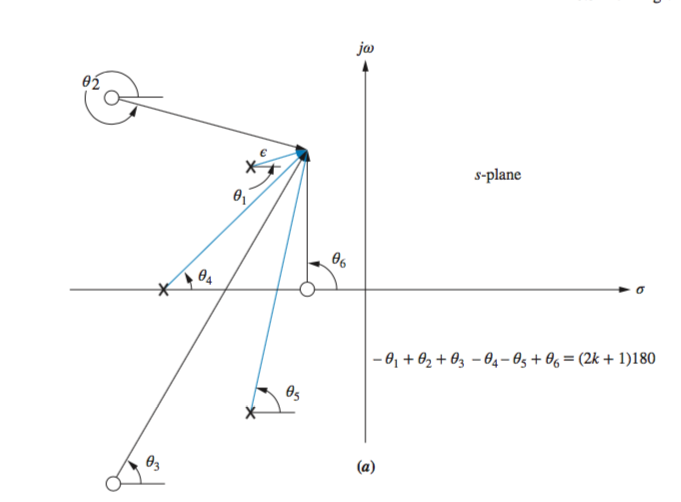
\includegraphics[width=300 px]{img/angles-pole} \\
    \end{center}    
    
    If we assume a point on the root locus $\epsilon$ close to a complex \textbf{zero}, the sum of angles drawn from all finite poles and zeros to this point is an odd multiple of 180$^\circ$. Except for the \textbf{zero} that is $\epsilon$ close to the point, we can assume all angles drawn from all other poles and zeros are drawn directly to the \textbf{zero} that is near the point. Thus, the only unknown angle in the sum is the angle drawn from the \textbf{zero} that is $\epsilon$ close. We can solve for this unknown angle, which is also the angle of arrival to this complex \textbf{zero}. \\ 

    $-\theta_1 + \theta_2 + \theta_3 - \theta_4 - \theta_5 + \theta_6 =…(2k+1)180^\circ$ \\ 
    
    \textit{or} \\ 

    $\theta_2 = \theta_1 - \theta_3 + \theta_4 + \theta_5 - \theta_6 -…(2k+1)180^\circ$ \\

    \begin{center}
        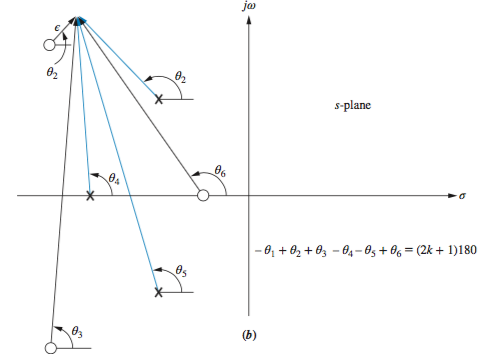
\includegraphics[width=300 px]{img/angles-zero} \\
    \end{center}  

    \subsection{Plotting and Calibrating the Root Locus}

    When locating points on the root locus and finding their specified gain, for example as it crosses the radial line representing 20\% overshoot, such as the below graph where $\zeta = 0.45$ \\ 

    Evaluating the graph at points along the line, and summing the angles from poles and zeros, it can be determined if a point is on the root locus if the angles are a multiple of 180$^\circ$.

    \begin{center}
        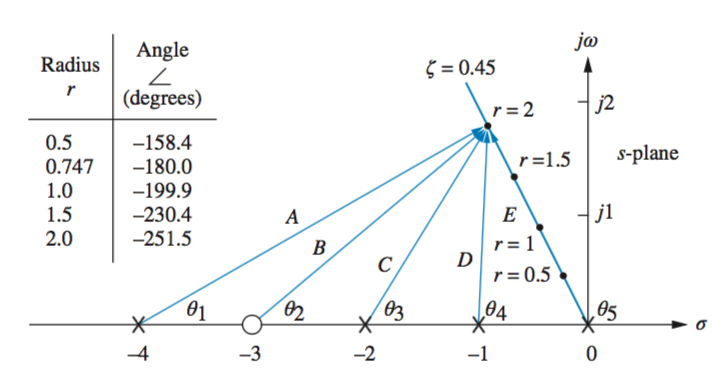
\includegraphics[width=300 px]{img/calibrating} \\
    \end{center}  

    \subsection{Generalized Root Locus}

    If finding the root locus of a system concerning a single parameter instead of gain $K$, an equivalent system can be used where the denominator is represented as $1 + p_1G(s)H(s)$. From the below system,\\ 
    \begin{center}
    $T(s) = \frac{KG(s)H(s)}{1 + KG(s)H(s)} = \frac{10}{s^2 + (p_1 +2)s + 2p_1 + 10} = \frac{10}{s^2 + 2s + 10 + p_1(s + 2)}$
    \end{center}

    \begin{center}
        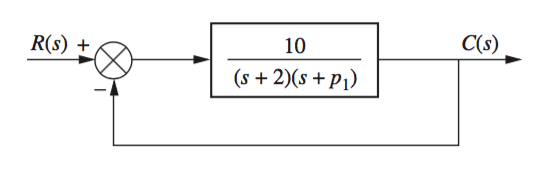
\includegraphics[width=300 px]{img/parameter1} \\
    \end{center}  

    \subsection{Positive Feedback Systems}

    $KG(s)H(s) = 1 =ˆ1 \angle k360^\circ \tab k = 0, 1, 2, 3... $

    \begin{enumerate}
        \item \textbf{Number of Branches} \\
        No change
        \item \textbf{Symmetry} \\
        No change
        \item \textbf{Real Axis Segments} \\
        On the real axis, the root locus for positive-feedback systems exists to the left of an \textbf{even} number of real-axis, finite open-loop poles and/or finite open-loop zeros.
        \item \textbf{Starting and Ending Points} \\
        The root locus for positive-feedback systems begins at the finite and infinite poles of $G(s)H(s)$ and ends at the finite and infinite zeros of $G(s)H(s)$.
        \item \textbf{Behavior at Infinity} \\        
        The root locus approaches straight lines as asymptotes as the locus approaches infinity. Further, the equations of the asymptotes for positive-feedback systems are given by the real-axis intercept, $\sigma_a$, and angle, $\theta_a$, as follows: \\
        \begin{center}
            $\sigma_a = \frac{\sum Finite Poles - \sum Finite Zeros}{\# Finite Poles - \# Finite Zeros}$ \\

            $\theta_a = \frac{k2\pi}{\# Finite Poles - \# Finite Zeros}$
        \end{center}    
        \end{enumerate}

    \section{Design via Root Locus}



    \section{Frequency Response Techniques}
    \section{Design via Frequency Response}
    
    \end{document}